\section{Analysis}

\subsection{Data Exploration and Visualization}
\label{subsec:Data_exploration_and_visualization}

The pictures have been automatically scraped from the online picture portals Flickr, Google Images and Yandex Images.

They represent single or multiple flowers under various angles, zoom, brightness conditions, life cycle stages, etc. 
\begin{center}
	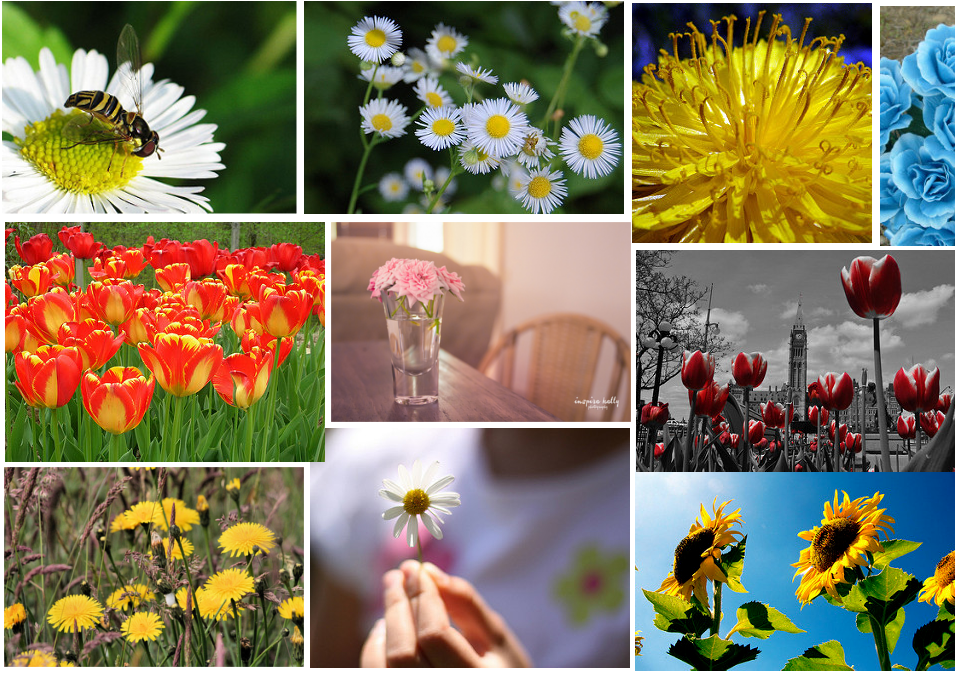
\includegraphics[scale=.25]{./sections/02_analysis/flowers_patchwork.png}
	\captionof{figure}{samples pictures}
\end{center}

The complete set of pictures distribution is as in Fig. \ref{fig:all-images-distribution}:

\begin{flushleft}
	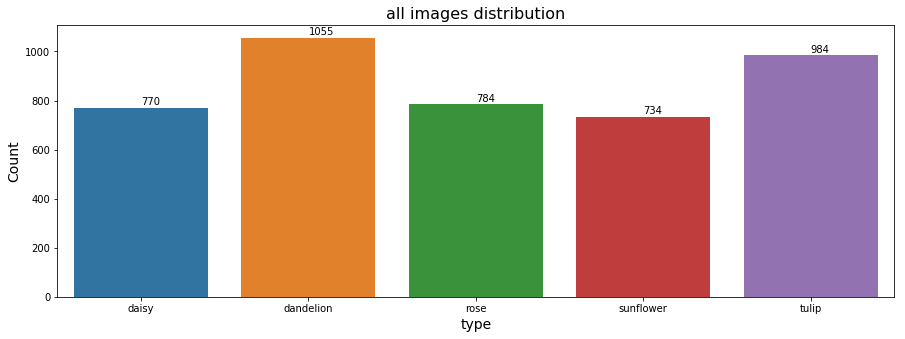
\includegraphics[scale=.5]{./sections/02_analysis/all_images_distribution}
	\captionof{figure}{All images distribution by label}
	\label{fig:all-images-distribution}
\end{flushleft}

We observe that the classes distribution is slightly unbalanced. There is an average of 865 pictures per classes to train the model, which is reasonably enough. The \textit{dandelion} class is the most represented with 1055 pictures. However, this flower variety has the particularity to be represented in 2 radically distinct state: the yellow flowers and the white "blow balls".
For this particular case, it is beneficial to have more sample to expect the model to be able to recognize both \textit{dandelion}'s aspects.  

Nevertheless, a significant number of pictures contains other subjects (persons, insects, other flowers, vase) or seem to be miss-classified. Such pictures can potentially impact negatively the model learning. A more detailed approach of the samples selection is described in chapter \fullref{subsec:Data_Preprocessing} 

\subsection{Algorithms and Techniques}

\subsubsection{pictures selection and split }

As already mentioned in the previous chapter, a large number of pictures seems inappropriate to train a model. A "blacklisting" approach will be put in place to discard them from the dataset.

On top of that, the selected pictures will be randomly split into three distinct training, validation and testing datasets. The random splitting is made in a stratified fashion in order to preserve the initial classes distribution in each set.

\subsubsection{image augmentation}

Image augmentation will be used to enrich the training and validation sets. This technique consist in modifying the original pictures in order to artificially generate more training samples. The modifications considered in this project consist of flipping, zooming, stretching or shrinking the images.

\subsubsection{Deep Convolutional Neural Network}

A deep convolutional network is a type of neural networks which architecture is designed in so called convolution layers. The principle of forward and back propagation common to neural networks remains. However the main particularity of a convolutional layer is to analyse the picture in small sub-regions and derive patterns from it. The sequencing of convolutional layers result in the identification of patterns increasingly complex. Consequently the patterns identified in the first layers are rather basic (points, stripes, lines,...) and generic to any pictures. On the contrary, the patterns identified by the last layers are more complex (objects, face attributes,...) and are specific to the problem addressed. 

\subsubsection{Transfer Learning}

The training of a full CNN requires significant computation resources and time. However, with Transfer Learning, it is possible to use pre-trained models. This techniques presents the double advantage to spare a significant amount of training time and to benefit from the quality of very deep architectures. 

Transfer learning consist of loading a pre-trained model, fix its weights, and replace the last layers in order to fit the new given problem.  
In this project, we will determine which among three models available in \texttt{Keras} module suits the best for flower classification. Those models have been trained on the \textit{ImageNet} dataset consisting of several million of labelled images representing thousands of objects. 

%A deep CNN has to be trained to recognize flowers variety from pictures. Rather than designing and training a full new CNN, we will take advantage of existing reference models by applying transfer learning. The weights of all convolutional layers of the base model will be loaded and frozen as-is. The top layers will be replaced by some of our own in order to specialize the mode to flowers types recognition. 

%An important part of this project will be dedicated to determine the most suitable base model to use.

\subsection{Benchmark}
\label{subsec:benchmark}

The benchmark for this project is the "Flowers Species Recognition" work from Yuning Chai, Victor Lempitsky and Andrew Zisserman from the University of Oxford in 2011 \cite{Chai_BiCos, Chai_BiCos_demo} . 

This two-steps approach consist of the segmentation of the pictures and the training of a kernelized SVM classifier. The best model reach a prediction accuracy of 80.0\% and is able to recognize flowers among 102 different variety.

The goal of this project is to reach at least this accuracy, however only 5 flower species are considered. 

